\documentclass[aspectratio=169]{beamer}

\usepackage{tikz}
\usepackage{listings}
\usepackage[utf8,latin1]{inputenc}
\usepackage[natbibapa]{apacite}
\usepackage{multirow}
\usepackage{color, colortbl}
\usepackage{tcolorbox}

\makeatletter \def\newblock{\beamer@newblock} \makeatother

\beamertemplatenavigationsymbolsempty
\setbeamertemplate{itemize items}[circle]
\setbeamertemplate{section in toc}[circle]
\mode<beamer>{\setbeamercolor{math text displayed}{fg=iwmgray}}
\setbeamercolor{block body}{bg=iwmorange!50!white}
\setbeamercolor{block title}{fg=white, bg=iwmorange}

\definecolor{iwmorange}{RGB}{255,105,0}
\definecolor{iwmgray}{RGB}{67,79,79}
\definecolor{iwmblue}{RGB}{60,180,220}
\definecolor{iwmgreen}{RGB}{145,200,110}
\definecolor{iwmpurple}{RGB}{120,0,75}

\setbeamercolor{title}{fg=iwmpurple}
\setbeamercolor{frametitle}{fg=iwmpurple}
\setbeamercolor{structure}{fg=iwmpurple}
\setbeamercolor{normal text}{fg=iwmgray}
\setbeamercolor{author}{fg=iwmgray}
\setbeamercolor{date}{fg=iwmgray}

\lstset{language = R,%
  basicstyle = \ttfamily\color{iwmgray},
  frame = single,
  rulecolor = \color{iwmgray},
  commentstyle = \slshape\color{iwmgreen},
  keywordstyle = \bfseries\color{iwmgray},
  identifierstyle = \color{iwmpurple},
  stringstyle = \color{iwmblue},
  numbers = none,%left,numberstyle = \tiny,
  basewidth = {.5em, .4em},
  showstringspaces = false,
  emphstyle = \color{red!50!white}}

\setbeamercolor{graybox}{bg=iwmgray!30}
\newenvironment{colbox}[1][\textwidth]%
  {\begin{beamercolorbox}[wd=#1, rounded=true, shadow=true]{graybox}}
  {\end{beamercolorbox}}

\AtBeginSection[]{
  \frame{
    \tableofcontents[sectionstyle=show/hide, subsectionstyle=show/show/hide]}}

% \setbeamertemplate{headline}{
%  \begin{beamercolorbox}{section in head}
%    \vskip5pt\insertsectionnavigationhorizontal{\paperwidth}{}{}\vskip2pt
%  \end{beamercolorbox}
% }

\setbeamertemplate{footline}{\vskip-2pt\hfill\insertframenumber$\;$\vskip2pt}

\title{Introduction to data simulation}
\author{Nora Wickelmaier\footnote{Parts of this slide set are a (modified)
version of slides accompanying the book by \citet{Strobl2024}}}
%\institute{Leibniz-Institut f\"ur Wissensmedien, T\"ubingen}
\date{Last modified: 2025-09-08}

\begin{document}

\begin{frame}{}
\thispagestyle{empty}
\titlepage
\end{frame}

% \begin{frame}{Outline}
% \tableofcontents
% \end{frame}

\begin{frame}{What are simulation studies used for?}
  \begin{itemize}
    \item Examining the properties of statistical methods
    \item Various applications of simulation studies
      \begin{itemize}
        \item Illustration or didactic explanation of properties of statistical
          methods (e.\,g.\ with Shiny Apps)
        \item Investigation of newly developed statistical methods for which
          theoretical properties are not yet known
        \item Investigation of properties of statistical methods that only hold
          asymptotically for realistic sample sizes
        \item Investigation of the impact of violated assumptions on statistical
          methods
        \item Power analyses for sample size planning
      \end{itemize}
    \item All these applications of simulation studies have as a common core
      that a simulation study represents an -- ideally well-planned --
      experiment
  \end{itemize}
  \vfill
  \flushright{\footnotesize\citet{Strobl2024}}
\end{frame}

\begin{frame}{Advantages of using simulated data}
  \begin{itemize}
    \item All properties of the data sets can be controlled
    \item Extreme scenarios can be examined, which are rare in real data
    \item Forces us to define (and think about) data generating process
    \item Data simulation (repeated sampling) is at the heart of hypothesis
      testing in the frequentist framework
  \end{itemize}
  \vfill
\end{frame}

\begin{frame}{Example simple data simulation}
  \begin{itemize}
    \item Let us look at a simple example and remind ourselves of the underlying
      concept of hypothesis testing after \citet{NeymanPearson33}
    \item We fit a simple regression line to predict stopping distance (in feet)
      of oldtimer cars with driving speed (in miles per hour)
    \item We fit a Null model that only predicts the mean
      \[
        y = \beta_0 + \varepsilon, ~~~\text{with } \varepsilon \sim N(0,
        \sigma^2_{\varepsilon})
      \]
      an a model that predicts distance with speed
      \[
        y = \beta_0 + \beta_1 \cdot x + \varepsilon, ~~~\text{with } \varepsilon
        \sim N(0, \sigma^2_{\varepsilon})
      \]
    \item We want to simulate the type I error rate for fitting a model
      including the slope $\beta_1$ when data were generated from the Null model
  \end{itemize}
\end{frame}

\begin{frame}[fragile]{Demonstration}
  {Hypothesis testing after Neyman and Pearson}
\begin{lstlisting}
lm0 <- lm(dist ~ 1, cars)       # H0
lm1 <- lm(dist ~ speed, cars)   # H1

nsim <- 1000
pval <- numeric(nsim)

for (i in 1:nsim) {
  sim <- simulate(lm0)$sim_1
  fit <- lm(sim ~ speed, cars)
  pval[i] <- summary(fit)$coef["speed", "Pr(>|t|)"]
}

# Type I error
mean(pval < 0.05)
\end{lstlisting}
\end{frame}

\begin{frame}{Structure of simulation studies}
  \begin{itemize}
    \item \citet{Strobl2024} recommend dividing code for simulation studies into
      three functions
      \begin{enumerate}
        \item \texttt{dgp} = data generating process
        \item \texttt{one\_simulation} = a single simulation run
        \item \texttt{simulation\_study} = complete simulation design
      \end{enumerate}
    \item This modular structure allows to easily extend the code and use it
      for different tasks
    \item Functions allow to combine individual work steps (promotes simplicity
      and clarity of the code)
    \item Functions are useful if the same work step is to be executed multiple
      times (e.\,g.\ data generation)
    \item Set of functions as a ``modular system''

  \end{itemize}
  \vfill
\end{frame}

\begin{frame}{Example of a simulation study}
  \begin{itemize}
    \item We are interested in estimating the slope coefficient $\beta_1$ in the
    simple linear regression model
  \item Possible questions we could ask are:
    \begin{enumerate}
      \item How much do the estimated slope coefficients deviate from the true
        slope coefficient for a given sample size?
      \item How does the accuracy of the estimation change when we alter the
        sample size?
    \end{enumerate}
    \item The model equation for a person $p$, with $p = 1,\dots, npers$, is:
      \[
        y_p = \beta_0 + \beta_1 \cdot x_p + \varepsilon_p, \hspace{0.2cm}
        \text{where} \hspace{0.1cm} \varepsilon_p \sim N(0, \sigma_{\varepsilon}^2)
      \]
    \item The model equation serves as a ``recipe'' for simulating data
  \end{itemize}
\end{frame}

\begin{frame}[fragile]{Data generating process}
  To generate data from the simple linear regression model, we need to specify:
  \begin{itemize}
    \item The parameters $\beta_0$ and $\beta_1$
    \item The variance $\sigma_{\varepsilon}^2$ or standard deviation
      $\sigma_{\varepsilon}$ of the error distribution
    \item The distribution from which we draw the $x$ values (commonly: uniform
      distribution or normal distribution)
    \item The sample size $npers$
  \end{itemize}
\begin{lstlisting}
npers <- 100
s_err <- 5
beta  <- c(1.5, 2.5),
\end{lstlisting}
\end{frame}

\begin{frame}[fragile]{Data generating process}
  \begin{itemize}
    \item Generating the random errors
      \begin{itemize}
    \item The simple linear regression model assumes $\varepsilon_p \sim N(0,
      \sigma_{\varepsilon}^2)$\\
    \item Random, normally distributed values can be generated in R using
      \texttt{rnorm()}:
      \end{itemize}
\begin{lstlisting}
err <- rnorm(n = npers, mean = 0, sd = s_err)
\end{lstlisting}
    \item Generating the $x$ and $y$ values
\begin{lstlisting}
x <- runif(n = npers, min = 0, max = 5)
beta <- c(1.5, 2.5)
y <- beta[1] + beta[2] * x + err
\end{lstlisting}
    \item Saving as a data frame
\begin{lstlisting}
dat <- data.frame(x = x, y = y)
\end{lstlisting}
  \end{itemize}
\end{frame}

\begin{frame}[fragile]{Data generating process}
  \begin{itemize}
    \item Model estimation to control data generation
\begin{lstlisting}
model <- lm(y ~ x, data = dat)
summary(model)
coef(model)
\end{lstlisting}
    \item We will now combine these steps into a function
\begin{lstlisting}
dgp <- function(npers, beta, s_err){
  x <- runif(n = npers, min = 0, max = 5)
  err <- rnorm(n = npers, mean = 0, sd = s_err)
  y <- beta[1] + beta[2] * x + err
  dat <- data.frame(x = x, y = y)
  return(dat)
}
\end{lstlisting}
  \end{itemize}
\end{frame}

% \begin{frame}[fragile]{Default values for functions}
% \begin{itemize}
%   \item Function arguments can be equipped with default values
% \begin{lstlisting}
% dgp <- function(npers = 100, beta = c(1.5, 2.5), 
%                 s_err = 5){
%   ...
% }
% \end{lstlisting}
%   \item Advantage: saves typing effort during programming
%   \item Disadvantage: if you are not aware of all default values, you may
%     generate data with undesirable properties
% \end{itemize}
% \vfill
% \end{frame}
% 
\begin{frame}[fragile]{Data generation with the \textup{\texttt{dgp}} function}
  \begin{itemize}
    \item If we execute the \texttt{dgp} function multiple times, different
      datasets are generated
  \end{itemize}
\begin{columns}[T]
\begin{column}{0.4\textwidth}
\centering
\begin{lstlisting}
dat <- dgp(npers = 100, 
        beta = c(1.5, 2.5),
        s_err = 5)
head(dat)

#           x         y
# 1 3.0105702 12.444386
# 2 0.9752196  9.033958
# 3 4.8322937 12.378318
# 4 3.2545276 18.024507
# 5 1.8353595  8.134339
# 6 4.9442961  9.418030
\end{lstlisting}
\end{column}

\begin{column}{0.4\textwidth}
\centering
\begin{lstlisting}
dat <- dgp(npers = 100, 
        beta = c(1.5, 2.5),
        s_err = 5)
head(dat)

#          x         y
# 1 2.081702 10.797706
# 2 1.272501  4.375452
# 3 1.508982  7.909477
# 4 4.474560 12.664724
# 5 3.103152 10.400254
# 6 4.588655  7.442873
\end{lstlisting}
\end{column}
\end{columns}
\end{frame}

\begin{frame}[fragile]{A single simulation run}
  \begin{itemize}
    \item We then create a function to run a single run of our simulation
    \item We want to simulate the estimated slope parameter $\beta_1$
\begin{lstlisting}
one_simulation <- function(npers, beta, s_err){
  dat <- dgp(npers = npers, beta = beta, s_err = s_err)
  model <- lm(y ~ x, data = dat)
  slope_est <- coef(model)[2]
  return(slope_est)
}

# Run one simulation
one_simulation(npers = 100, beta = c(1.5, 2.5), s_err = 5)
\end{lstlisting}
  \end{itemize}
\end{frame}

\begin{frame}[fragile]{500 simulation runs}
  \begin{itemize}
    \item We can now use a for-loop to repeat our data simulation
\begin{lstlisting}
niter <- 500
slope_est <- rep(NA, niter)
for(i in 1:niter) {
  slope_est[i] <- one_simulation(npers = 100, 
                                 beta = c(1.5, 2.5), 
                                 s_err = 5)
}
\end{lstlisting}
\item As expected, the estimated slopes scatter around the specified true value
\begin{lstlisting}
boxplot(slope_est)
abline(h = 2.5, lty = 2)
\end{lstlisting}
  \end{itemize}
\end{frame}

\begin{frame}[fragile]{Complete simulation design}
  \begin{itemize}
    \item The last step is to write a function for a complete simulation study
      design
    \item The factors that we want to investigate (e.\,g.\ different sample
      sizes, different variation in the data) are arguments for this function
\begin{lstlisting}
simulation_study <- function(niter, npers, beta, s_err){
  prs <- expand.grid(i = 1:niter, npers = npers, 
                     s_err = s_err)
  slope_est <- rep(NA, nrow(prs))
  for(i in 1:nrow(prs)) {
    slope_est[i] <- one_simulation(npers = prs$npers[i],
                                   beta = beta,
                                   s_err = prs$s_err[i])
  }
  return(cbind(prs, slope_est))
}
\end{lstlisting}
  \end{itemize}
\end{frame}

\begin{frame}[fragile]{The \texttt{expand.grid} function}
\begin{lstlisting}
niter <- 2
factor_1 <- c("a", "b")
factor_2 <- c(5, 10)
expand.grid(i = 1:niter, variant = factor_1, quantity = factor_2)
#   i variant quantity
# 1 1       a       5
# 2 2       a       5
# 3 1       b       5
# 4 2       b       5
# 5 1       a      10
# 6 2       a      10
# 7 1       b      10
# 8 2       b      10
\end{lstlisting}
\end{frame}

\begin{frame}[fragile]{Conducting the simulation}
  \begin{itemize}
    \item For each combination of factor levels of \texttt{npers} and
      \texttt{s\_err} we perform 500 simulation runs ($500 \times 2 \times 2 =
      2000$
      runs)
\begin{lstlisting}
sim_results <- simulation_study(niter = 500,
                                npers = c(100, 200),
                                beta = c(1.5, 2.5),
                                s_err = c(5, 10))
head(sim_results)
#   i npers s_err slope_est
# 1 1   100     5  2.552509
# 2 2   100     5  2.477369
# 3 3   100     5  3.509792
# 4 4   100     5  3.464987
# 5 5   100     5  3.154455
# 6 6   100     5  3.027992
\end{lstlisting}
  \end{itemize}
\end{frame}

\begin{frame}[fragile]{Graphical presentation of results}
  {Distribution of estimated slope coefficients around the true value 2.5}
  \begin{columns}
    \begin{column}{0.5\textwidth}
      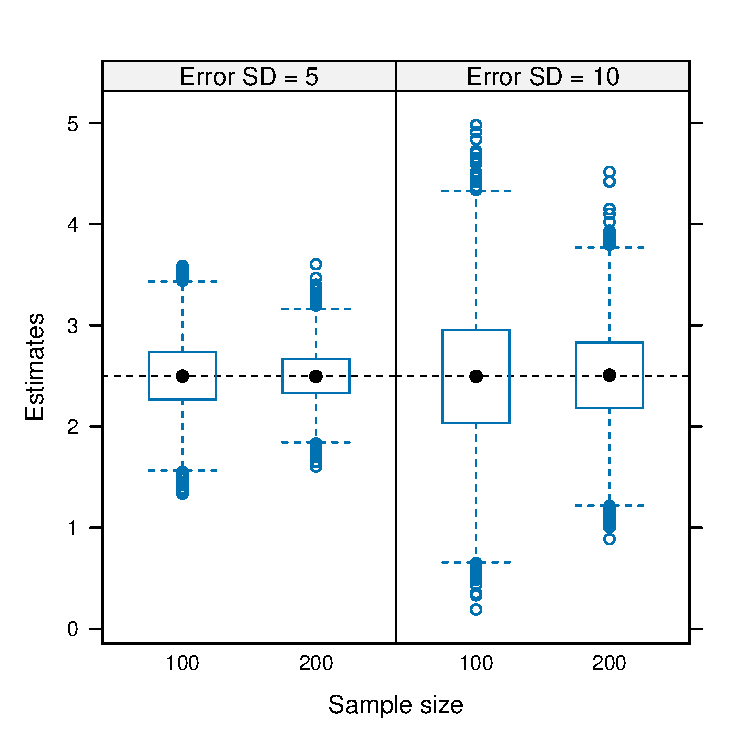
\includegraphics[scale = .57]{../figures/boxplot_simstudy_example1}
    \end{column}
    \begin{column}{0.555\textwidth}
\begin{lstlisting}
library("lattice")
bwplot(slope_est ~ npers | s_err, 
       data = sim_results,
       xlab = "Sample size",
       ylab = "Estimates")
\end{lstlisting}
    \end{column}
  \end{columns}
\end{frame}

\appendix
\begin{frame}{References}
%\begin{frame}[allowframebreaks]{References}
%\renewcommand{\bibfont}{\footnotesize}
\bibliographystyle{apacite}
\bibliography{../lit}
\end{frame}

\end{document}

